\documentclass{article}

% Language setting
% Replace `english' with e.g. `spanish' to change the document language
\usepackage[german]{babel}
\usepackage{xcolor}

% Set page size and margins
% Replace `letterpaper' with `a4paper' for UK/EU standard size
\usepackage[letterpaper,top=2cm,bottom=2cm,left=3cm,right=3cm,marginparwidth=1.75cm]{geometry}

% Useful packages
\usepackage{amsmath}
\usepackage{graphicx}
\usepackage[colorlinks=true, allcolors=blue]{hyperref}
\usepackage{float}

\title{Software Entwicklung 1}
\author{Asha Schwegler}

\begin{document}
\maketitle


\section{Software Engineering}

\begin{itemize}
    \item Herstellung / Entwicklung von Software
    \item Organisation und Modellierung (Zugehörigen Datenstrukturen, Bettrieb von Softwaresystemen)
    \item Strukturiertes Projektplan f. Entwicklung
    \item Unterteilung Entwicklungsprozess
    \begin{itemize}
        \item Schritte (überschaubar, zeitlich und inhaltlich begrenzt)
        \item Phasen
        \item Meilensteine
    \end{itemize}
    \item Disziplinen während Entwicklungsprozess sind verzahnt.
    
\end{itemize}

\paragraph{Disziplinen}
\begin{itemize}
    \item \textbf{Kerndisziplinen}
    \begin{itemize}
        \item Anforderungsanalyse
        \item Softwarearchitekur und Design
        \item Implementierung / Test
        \item Softwareverteilung
        \item Softwareeinführung
        \item Wartung / Pflege
    \end{itemize}
    \item \textbf{Unterstützungsdisziplinen}
    \begin{itemize}
        \item Projektmanagement
        \item Konfigurationsmanagemdnt
        \item Risikomanagement
    \end{itemize}
\end{itemize}


\section{Prozess und Prozess-Modell}
\begin{itemize}
    \item Prozess
    \begin{itemize}
        \item Beschreibung Aktivitäten, Rollen und Artefakte(Informationen)
        \item Software-Entwicklung und Wartung
    \end{itemize}
    \item Prozessmodell
    \begin{itemize}
        \item Präskriptives Modell (Vorgehensmodell und Organisationsstrukturen)
        \item Planung und Lenkung
        \item Unified Process, V-Modell, Scrum,...
    \end{itemize}
\end{itemize}
\subsection{Vorgehensmodelle}
\begin{itemize}
    \item Code and Fix
    \item Wasserfallmodell
    \item Iterative und inkrementelle Modelle
\end{itemize}

\paragraph{Code and Fix}
\begin{itemize}
    \item Definition
    \begin{itemize}
        \item Codierung / Korrektur im Wechsel mit Ad-hoc Tests
    \end{itemize}
    \item Vorteile
    \begin{itemize}
        \item Schnell vorankommen
        \item Schnelle Ergebnisse
        \item Einfache Tätigkeiten (Codieren, Testen, Fixen)
    \end{itemize}
    \item Nachteile
    \begin{itemize}
        \item Schlecht planbar und keine Unterstützung im Team
        \item Aufwand hoch für Korrekturen
        \item Sclecht wartbare Software
    \end{itemize}
\end{itemize}

\paragraph{Wassefallmodell}
\begin{itemize}
    \item Definition
    \begin{itemize}
        \item Folge von Aktivitäten/Phasen, gekoppelt durch Teilergebnisse (Dokumente). Reihenfolge ist fest definiert.
    \end{itemize}
    \item Vorteile
    \begin{itemize}
        \item hohe Planbarkeit
        \item Klare Aufteilung der SWE (Analyse, Design, Test,...)

      \end{itemize}
    \item Nachteile
    \begin{itemize}
        \item Schlechtes Risikomanagement (Lösungskonzept nur auf Papier validiert)
        \item Anforderungen zu Beginn nie alle bekannt
    \end{itemize}
\end{itemize}

\paragraph{Iterativ-inkrementelle Modelle}
\begin{itemize}
    \item Definition
    \begin{itemize}
        \item Geplante und kontrollierte Iterationen inkrementell entwickelt
    \end{itemize}
    \item Vorteile
    \begin{itemize}
        \item Flexibles Modell bei unklaren Anforderungen
        \item Gutes Risikomanagement (Mitarbeiter und Technologie)
        \item Frühe Einsetzbarkeit der Software und Feedback
    \end{itemize}
    \item Nachteile
    \begin{itemize}
        \item Upfront Planbarkeit hat Grenzen (Funktionalität, Zeit und Kosten)
        \item Braucht Involvierung und Steuerung durch den Kunden über ganze Projektdauer
    \end{itemize}
\end{itemize}


\subsection{Agile SWE}
\begin{itemize}
    \item Basiert auf iterativ-inkrementellen Prozessmodell
    \item Fokussiert auf gut dokumentierten und getesteten Code statt auf ausführlicher Dokumentation
    \item Sammlung von Ideen SWE Prozess flexibler und schlanker zu machern
    \item Adressiert bekannten Probleme bei klassischen Software-Prozessmodellen
\end{itemize}

\paragraph{Strategie}
\begin{itemize}
    \item Definierte Prozesskontrolle
    \begin{itemize}
        \item Planung am Anfang, Prozess gesteuert und überwacht
        \item Geeignet für gut planbare Problemstellungen
        \item Strategie: Steuerung
    \end{itemize}
    \item Empirische Prozesskontrolle (Agil)
    \begin{itemize}
        \item Nur Grobplanung am Anfang
        \item Prozess fortlaufend überwacht
        \item Rollende Planung
        \item Geeignet für komplexe Problemstellungen
        \item Strategie: Regelung, Deming-Cycle (Plan-Do-Check-Act)
    \end{itemize}
\end{itemize}

\begin{figure}[H]
\centering
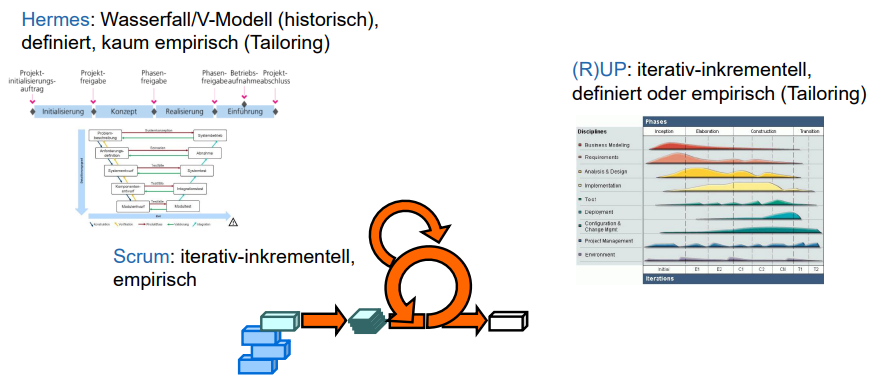
\includegraphics[width=0.3\textwidth]{Resources/Images/CharaktersierungProzessmodellen.png}
\caption{\label{fig:CharaktersierungProzessmodellen}CharaktersierungProzessmodellen}
\end{figure}

\section{Modellierung}

\textbf{Modell: } Abbild oder Vorbild für ein zu schaffendes  Gebilde.\\
\textbf{Original: } Abgebildete oder zu schaffende Gebilde \\

\begin{itemize} 
    \item \textbf{Modellierung} 
    \begin{itemize}
        \item Software selbst ein Modell
        \item Anforderungen = Modelle der Lösung
        \item Tesfälle = Modelle Korrektes Funktionieren des Codes
    \end{itemize}

\end{itemize}

\subsection{UML}

\begin{figure}[H]
\centering
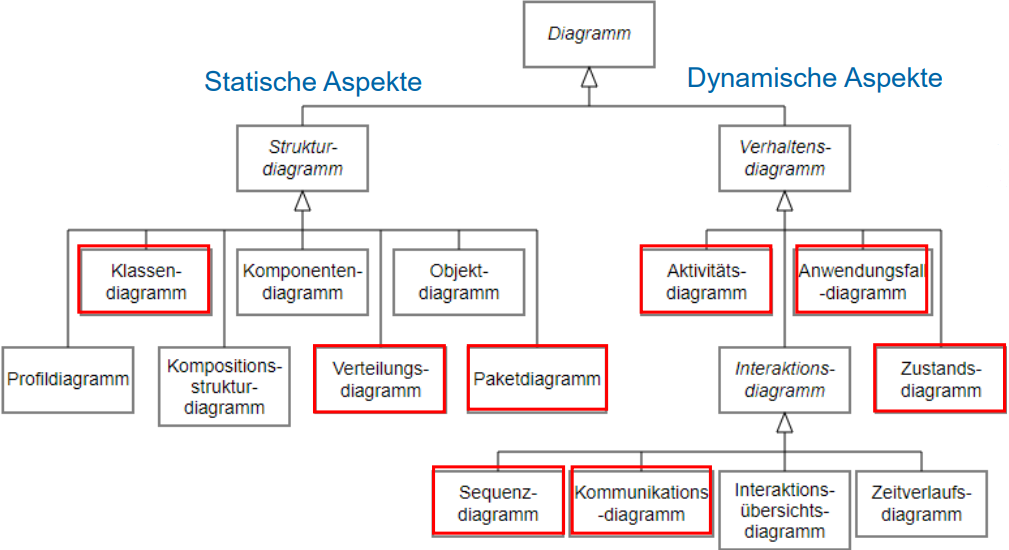
\includegraphics[width=0.3\textwidth]{Resources/Images/UML_Diagramme.png}
\caption{\label{fig:Guetereinteilung}Guetereinteilung.}
\end{figure}

\subsubsection{Gebrauch der UML}
\begin{itemize}
	\item UML as a sketch
	\begin{itemize}
		\item Informell, unvollständig
		\item Bevorzugt von agile Community
	\end{itemize}
	\item UML as blueprint
	\begin{itemize}
		\item Detallierte Analyse und Design-Diagramme für Code  
		\item Forward - und Reverse-Engineering
	\end{itemize}
	\item UML as a Programming Language
	\begin{itemize}
		\item Komplette, ausführbare Spezifikation eines Software-Systems in UML
		\item MDA-Tools zur Modellierung und Generierung
	\end{itemize}

\end{itemize}

\section{Wesentliche Artefakte}
\begin{itemize}
	\item Anfoderungsanalyse
	\begin{itemize}
		\item Funktionale Anforderungen mit Use Cases
		\item Qualitätsanforderungen und Randbedingungen
	\end{itemize}
	\item Design
	\begin{itemize}
		\item Softwarearchitektur
		\item Use Case Realisierung (Statische und dynamische Modelle)
	\end{itemize}
	\item Implementation
	\begin{itemize}
		\item Quellcode (inkl.Javadoc)
	\end{itemize}
	\item Testing
	\begin{itemize}
		\item Unit-Tests
		\item Integrations- und Systemtests
	\end{itemize}
\end{itemize}

\subsection{Überblick Anforderungsanalyse}

\begin{itemize}
	\item \textbf{User Research}
	\begin{itemize}
		\item Personas 
		\item Szenarien
		\item Contextual Inquiry
	\end{itemize}
	\item Sketching und Prototyping
	\item \textbf{Use Cases}
	\begin{itemize}
		\item Ableiten und Modellieren
		\item Detaillierung (UML-Use-Case-Diagramm, Use-Case-Spezifikation, UI-Sketching)
	\end{itemize}
	\item \textbf{Qualitätsanforderungen, Randbedingungen} erheben
	\item \textbf{Domänenmodell}
	\begin{itemize}
		\item Konzeptuelles UML-Klassendiagramm 
	\end{itemize}
	\item \textbf{objektorientierten Analyse(OOA)} 
	\begin{itemize}
		\item Objekte/Konzepte in dem Problembereich zu finden und zu beschreiben
	\end{itemize}
\end{itemize}

\subsection{Überblick Design}
\begin{itemize}
	\item \textbf{Softwarearfchitektur}
	\begin{itemize}
		\item UML-Paketdiagramm
		\item UML-Deploymentdiagramm
	\end{itemize}
	\item \textbf {Use-Case-Realisierung und Klassendesign}
	\begin{itemize}
		\item UML-Klassendiagramm
		\item UML-Sequenzdiagramm
		\item UML-Kommunikationsdiagramm
		\item UML-Zustandsdiagramm
		\item UML-Aktivitätsdiagramm
	\end{itemize}
	\item Entwurf \textbf{Design Patterns}
	\item \textbf{Objektorientierten Design (OOD)}
	\begin{itemize}
		\item Geeignete Softwareobjekte und ihr Zusammenwirken definieren
	\end{itemize}
\end{itemize}

\subsection{Überblick Implementation}
\begin{itemize}
	\item \textbf{Code}
	\begin{itemize}
		\item Umsezung Design in entspr. OOP-Sprache
	\end{itemize}
	\item \textbf{Refactoring}
	\begin{itemize}
		\item Code smells aufdecken und verbessern
	\end{itemize}
	\item \textbf{laufende Dokumentierung}
	\begin{itemize}
		\item Quellcode
	\end{itemize}
\end{itemize}

\subsection{Überblick Testing}
\begin{itemize}
	\item \textbf{Unit-Tests}
	\begin{itemize}
		\item Laufendes Design und Implementierung
	\end{itemize}
	\item \textbf{Teststufen Integration und System}
	\begin{itemize}
		\item Planung, Design und Durchführung
	\end{itemize}
	\item \textbf{Dokumentation}
	\begin{itemize}
		\item Testkonzept und Test
	\end{itemize}
\end{itemize}


\section{Usability und User Experience (UX)}

\begin{figure}[H]
\centering
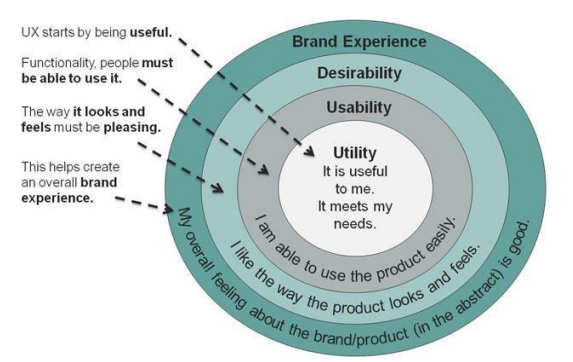
\includegraphics[width=0.3\textwidth]{Resources/Images/Usability.png}
\caption{\label{fig:Usability}Usability.}
\end{figure}


\subsection{Usability}
\textbf{Definition: } Effektivität, Effizienz, Zufriedenheit -> Ziele erreichen im spezifischen Kontext \\

\begin{itemize}
	\item \textbf{4 wichtige Aspekte}
	\begin{itemize}
		\item Benutzer
		\item Seine Ziele/Aufgaben
		\item Sein Kontext
		\item Softwaresystem (inkl.UI)
	\end{itemize}
\end{itemize}


\subsection{Usability Engineering}

\textbf{Ziel: } Software entwickeln, die drei Anfroderungen erfüllt

\begin{itemize}
	\item \textbf{Drei Anforderungen: }
	\begin{itemize}
		\item Effektivität
		\begin{itemize}
			\item Aufgaben vollständig erfüllen
			\item Genauigkeit
		\end{itemize}
	
		\item Effizienz
		\begin{itemize}
			\item Mit minimalem Aufwand (Mental, Physisch, Zeit)
		\end{itemize}
					\item Zufriedenheit 
		\begin{itemize}
			\item \textbf{Minimum: } nicht verärgert
			\item \textbf{Normal: } Zufrieden
			\item \textbf{Optimal: } Erfreut
		\end{itemize}

	\end{itemize}

\end{itemize}


\subsection{Usability Anforderungen}

\begin{itemize}
	\item \textbf{7 Anforderungen:}
	\begin{itemize}
		\item Aufgabengemessenheit
		\item Lernförderlichkeit
		\item Individualisierbarkeit
		\item Erwartungskonformität
		\item Selbstbeschreibungsfähigkeit
		\item Steuerbarkeit
		\item Fehlertoleranz
	\end{itemize}
\end{itemize}


\subsubsection{Aufgabenangemessenheit}
\begin{itemize}
	\item Minimale Anz. Schritte f. Aufgabe
	\item Nur wichtige Informationen
	\item Kontextabhängige Hilfe
	\item Minimale Anz. Benutzereingaben
	\begin{itemize}
		\item Jede Eingabe nur 1x
		\item Standardwerte
		\item Liste vordefinierter Werte (z.B Länder)
		\item Ableitbare Eingaben vorschlagen
	\end{itemize}
\end{itemize}

\subsubsection{Selbstbeschreibungsfähigkeit}
\begin{itemize}
	\item Benutzer ausreichend informieren

	\begin{itemize}
		\item Wo er ist
		\item Was er tun soll / kann
		\item Wie er es tun soll (Formate, Werte)
	\end{itemize}
	
	\item Begriffe des Benutzers verwenden (Labels, Fehlermeldungen)
	\item Affordanzen

\end{itemize}


\subsubsection{Kontrolle}

\begin{itemize}
	\item Mit Interaktion Benutzer steuern
	\begin{itemize}
		\item Initiative, Tempo
		\item Dialogfluss
		\item Darstellungsformate
		\item Inputmodalität (Maus, Tastatur, Touch, Sprache)
	\end{itemize}
	
	\item Benutzeraktionen rückgängig machen können
	\item Benutzeraktionen jeder Zeit abbrechen können
\end{itemize}

\subsubsection{Erwartungskonformität}
\begin{itemize}
	\item Bezüglich
	\begin{itemize}
		\item Design
		\item Interaktion
		\item Struktur
		\item Komplexität
		\item Funktionalität
	\end{itemize}
	\item Konsistenz
	\begin{itemize}
		\item Terminologie
		\item Verhalten (Reihenfolge Aktionen, Änderungen)
		\item Informationsdarstellung (Platzierung, Wortwahl)
	\end{itemize}
\end{itemize}

\subsubsection{Fehlertoleranz}
\begin{itemize}
	\item Benutzerfehler vermeiden
	\begin{itemize}
		\item Klar kommunizieren (Erwarteter Input, Funktionen aktiv resp. sinnvoll)
	\end{itemize}
	\item Benutzereingaben vor Aktion überprüfen
	\item Nicht unbedingt beim Tippen
	\item Benutzer helfen
	\begin{itemize}
		\item Fehler zu erkennen
		\item Ursache zu verstehen
		\item Aus Fehlerzustand zu kommen
	\end{itemize}
	\item Einfache Korrektur
	\item Kein Datenverlust
\end{itemize}

\subsubsection{Individualisierbarkeit}
\begin{itemize}
	\item System anpassbar sein:
	\begin{itemize}
		\item Know-How
		\item Sprache
		\item Kultur
		\item Benutzer mit Einschränkungen
	\end{itemize}	
\end{itemize}

\subsubsection{Lernförderlichkeit}
\begin{itemize}
	\item Informationen über unterliegende Konzepte und Regeln anbieten
	\begin{itemize}
		\item Um mentales Modell anzugleichen
		\item Nur auf Verlangen des Users
		\item eifache Tasks ohne Vorkentnisse
		\item komplexere Konzepte bei der Verwendung zu erlernen
	\end{itemize}
\end{itemize}

\section{User-Centered Design (UCD)}
\begin{figure}[H]
\centering
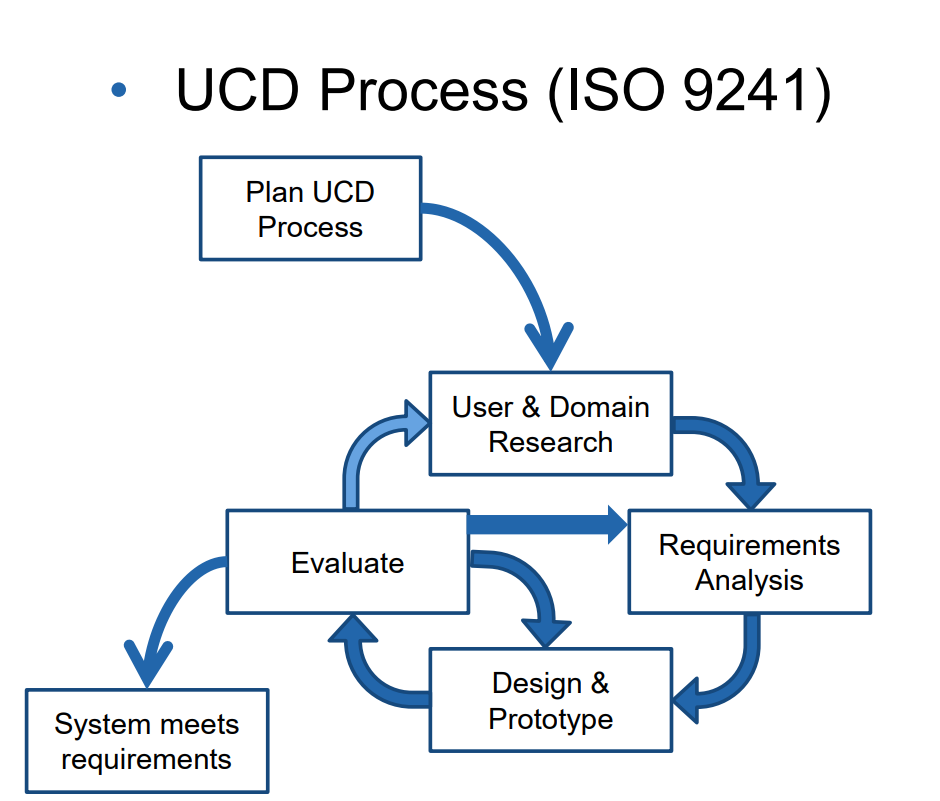
\includegraphics[width=0.3\textwidth]{Resources/Images/UCD_Process.png}
\caption{\label{fig:UCDProcess} UCDProcess}
\end{figure}


\subsection{User \& Domain Research}
\begin{itemize}
	\item \textcolor{red} {\textbf{Ziele bez. Benutzer:}}
	\begin{itemize}
		\item Wer ist Benutzer
		\item Was ist die Arbeit (Aufgaben, Ziele)
		\item Wie sieht Arbeitsumgebung aus
		\item Was wird gebraucht um Ziele zu erreichen
	\end{itemize}
	\item Welche Sprache, Begriffe
	\item Normen (organisatorisch, kulturell, sozial)
	\item Pain Points (Brüche, Workarounds)
	\item Für mobile Apps:
	\begin{itemize}
		\item Nutzungskontext
		\begin{itemize}
			\item Wo wird App benutzt (Umgebung)
			\item Wann wird App benutzt (Tageszeit, involvierte Personen, Randbedingungen)
			\item Warum wird App benutzt (Nutzen, Motivation, Trigger)
		\end{itemize}
	\end{itemize}
	\item \textcolor{red} {\textbf{Ziele bez. Domäne:}}
	\begin{itemize}
		\item Buisiness der Firma verstehen
		\item Domäne verstehen (Sprache, Wichtigste Konzepte, Prozesse)
	\end{itemize}
	
\end{itemize}




\subsubsection{GUI Design Process}
\paragraph{Methoden User \& Domain Research}
\begin{itemize}
	\item Contextual Inquiry
	\item Interviews
	\item Beobachtung
	\item Fokusgruppen
	\item Umfragen
	\item Nutzungsauswertung
	\item Desktop Research (Dokumentenstudium, Mitbewerber)
\end{itemize}


\subsubsection{Wichtige Artekfakte}
\begin{itemize}
	\item \textcolor{pink}{\textbf{Personas}}
	\item \textcolor{pink}{\textbf{Usage-Szenarien}}
	\begin{itemize}
		\item Kurze Geschichte
		\begin{itemize}
			\item \textcolor{green} {Usage Szenarien}
			\begin{itemize}
				\item aktuelle Situation
				\item in User and domain research verwendet
			\end{itemize}
			\item \textcolor{green} {Kontextszenarien}
			\begin{itemize}
				\item Zukünftige gewünschte Situation
				\item in Anforderungsanalyse verwendet
			\end{itemize}
		\end{itemize}
		
	\end{itemize}
	\item \textcolor{pink}{\textbf{Mentales Modell}}
	\item \textcolor{pink}{\textbf{Domänenmodell}}
	\item \textcolor{pink}{\textbf{Stakeholder Map}}
	\begin{figure}[H]
	\centering
	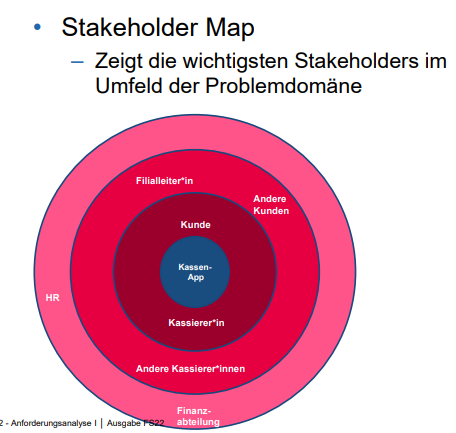
\includegraphics[width=0.3\textwidth]{Resources/Images/Stakeholdermap.png}
	\caption{\label{fig:Stakeholdermap} Stakeholdermap}
	\end{figure}
	\item \textcolor{pink}{\textbf{Service Blueprint/Geschäftsprozessmodell}}
	\begin{figure}[H]
	\centering
	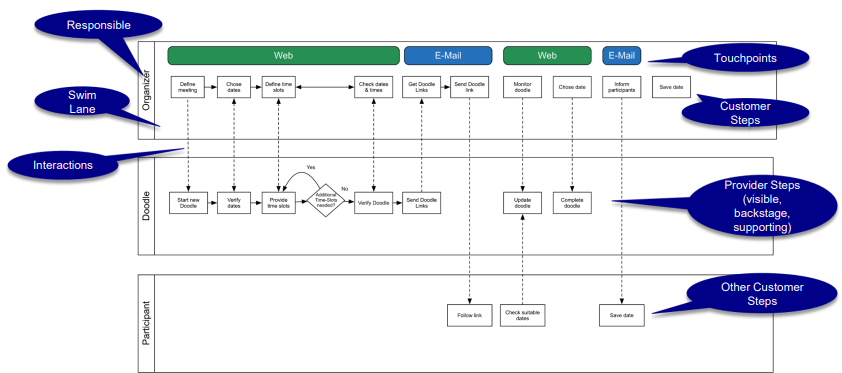
\includegraphics[width=0.3\textwidth] {Resources/Images/Blueprint.png}
	\caption{\label{fig:Blueprint}Blueprint}
	\end{figure}
	
\end{itemize}

\subsection{Anforderungsanalyse}

\textbf{Ziel:}\\
\begin{itemize}
	\item Ausgehend von den Resultaten des UCD -> User-Anforderungen ableiten:
	\begin{itemize}
		\item Funktionale Abläufe, Interaktionen 
		\begin{itemize}
			\item \textcolor {gray} {\textbf{Kontextszenarien}}
			\item \textcolor {gray} {\textbf{Storyboards}}
			\item \textcolor {gray} {\textbf{UI-Skizzen}}
			\item \textcolor {gray} {\textbf{Use cases}}
		\end{itemize}
		\item Konzepte, Beziehungen, Quantitäten
		\begin{itemize}
			\item \textcolor {gray} {\textbf{Kontextszenarien}}
		\end{itemize}
		\begin{itemize}
			\item \textcolor {gray} {\textbf{FURPS-Modell (Functionality, Usability, Reliability, Performance, Supportablility}}
		
		\end{itemize}				
		
	\end{itemize}
\end{itemize}


\subsubsection{Use Cases}

\begin{itemize}
	\item Akteur
	\begin{itemize}
		\item Primärakteur
		\item Unterstützender Akteur
		\item Offstage-Akteur
	\end{itemize}
	\item Keine Kann-Formulierungen
	\item 3 Ausprägungen:
	\begin{itemize}
		\item Kurz
		\begin{itemize}
			\item Titel + 1 Absatz (Standardablauf)
		\end{itemize}
		\item Informell
		\begin{itemize}
			\item Titel + Informelle Beschreibung (können mehrere Absätze sein, beschreibt auch Varianten)
		\end{itemize}
		\item Vollständig
		\begin{itemize}
			\item Titel + alle Schritte und alle Varianten im Detail
			\item UC-Name
			\item Umfang
			\item Ebene
			\item Primärakteur
			\item Stakeholders und Interessen
			\item Vorbedingungen
			\item Erfolgsgarantie/Nachbedingungen
			\item Standardablauf
			\item Erweiterungen
			\item Spezielle Anforderungen
			\item Liste der Technik und Datavariationen
			\item Häfigkeit des Auftretens
			\item Verschiedenes
		\end{itemize}
		\item Notation = Nomen + Verb
	\end{itemize}
\end{itemize}


\title {Use-Case-Diagramm}

\begin{figure}[H]
	\centering
	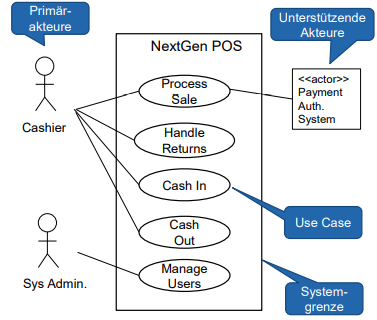
\includegraphics[width=0.3\textwidth] {Resources/Images/UseCaseDiagramm.png}
	\caption{\label{fig:UseCaseDiagramm}UseCaseDiagramm}
	\end{figure}


\title {Zusätzliche Beziehungen im Use Case Diagramm}

\begin{figure}[H]
	\centering
	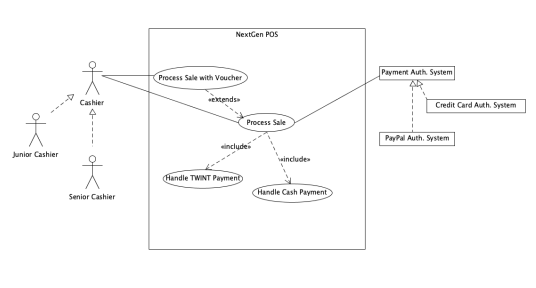
\includegraphics[width=0.3\textwidth] {Resources/Images/UseCaseDiagramm2.png}
	\caption{\label{fig:UseCaseDiagramm2}Zusätzliche Beziehungen UseCaseDiagramm}
	\end{figure}


\subsubsection{UML Sequenzdiagramm (SSD)}


\begin{figure}[H]
	\centering
	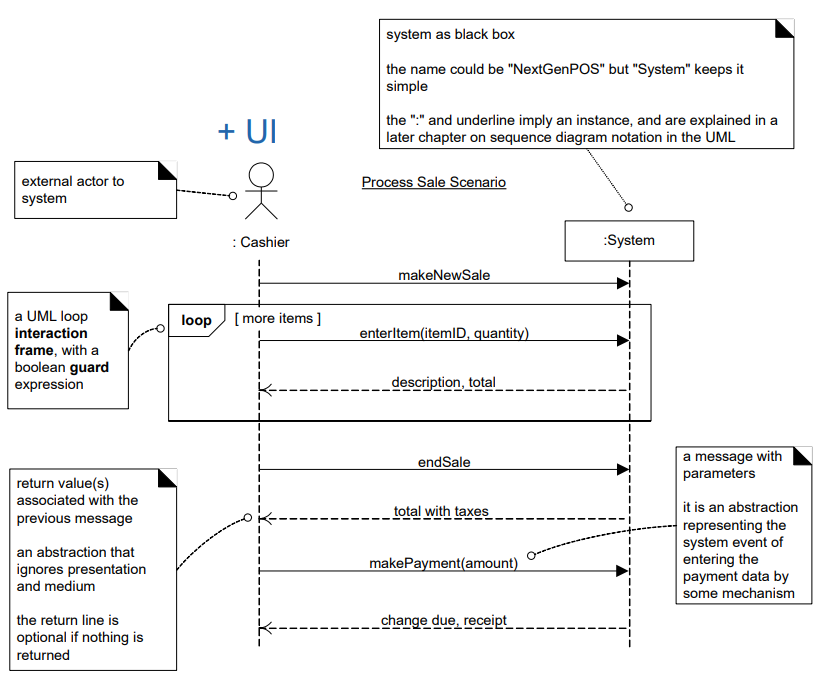
\includegraphics[width=0.3\textwidth] {Resources/Images/Systemsequenzdiagramm.png}
	\caption{\label{fig:Systemsequenzdiagramm}Zusätzliche Beziehungen Systemsequenzdiagramm}
	\end{figure}
	
\title {SSD zwischen zwei Systemen}
\begin{figure}[H]
	\centering
	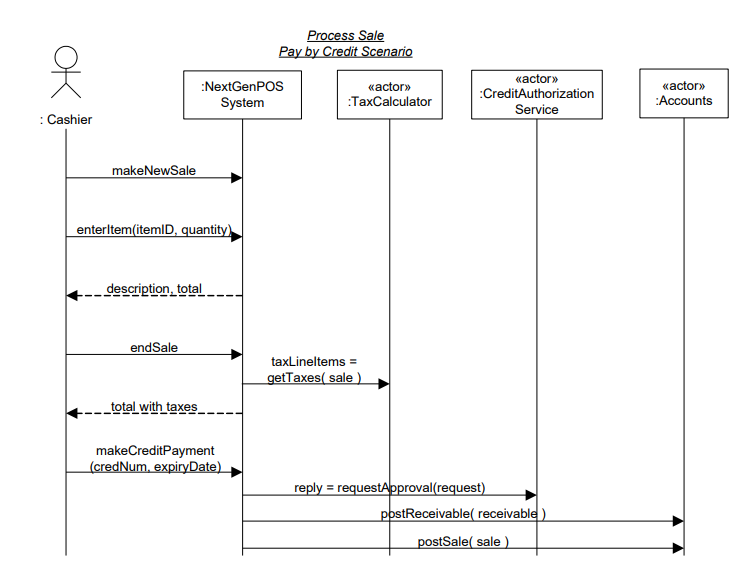
\includegraphics[width=0.3\textwidth] {Resources/Images/SSD2.png}
	\caption{\label{fig:SSD2}Zusätzliche Beziehungen Systemsequenzdiagramm zwischen zwei Systeme}
	\end{figure}

\paragraph{System Operation}
\begin{itemize}
	\item Formal wie ein Methodenaufruf
	\begin{itemize}
		\item Treffender Name
		\item Evt. mit Parametern
		\item Durchzogener Pfeil für Methodenaufruf
		\item Rückgabewert (Kann fehlen falls unwichtig, Gestrichelte Linie weil Update des UI)
		\item Definieren API des Systems
	\end{itemize}

\end{itemize}

\subsubsection{Operation Contract}

\textbf{Definition: } Spezifiziert (System)Operation \\

\begin{itemize}
	\item Name plus Parameterliste
	\item Vorbedingung (Was muss zwingend erfüllt sein damit Systemoperation aufgerufen werden kann)
	\item Nachbedingung
	\begin{itemize}
		\item Was hat sich alles geändert nach Ausführung (Erstellte / gelöschte Instanzen, Assoziationen, geänderte Attribute)
		\item basierend auf Domänenmodell
	\end{itemize}
\end{itemize}

\begin{figure}[H]
	\centering
	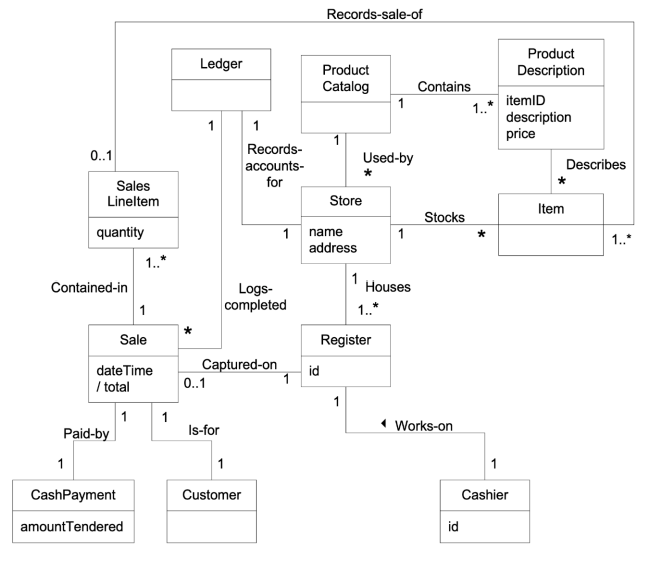
\includegraphics[width=0.3\textwidth] {Resources/Images/OperationContract.png}
	\caption{\label{fig:OperationContract}OperationContract}
	\end{figure}



\subsubsection{Zusätzliche Anforderungen}
\begin{itemize}
	\item Funktionale
	\item Nicht-Funktionale
\end{itemize}


\paragraph{Formulierung}

\begin{itemize}
	\item Anforderungstatements
	\begin{itemize}
		\item Als Anforderung formuliert
		\item messbar/verifizierbar
	\end{itemize}
	\item So wenig wie nötig
	\begin{itemize}
		\item Nur diejenige, die begründet gefordert werden
		\item Keine ersten Lösungsideen als Forderungen
	\end{itemize}
\end{itemize}


\paragraph{Checkliste FURPS+}

\begin{itemize}
	\item \textbf Functionality
	\begin{itemize}
		\item Features, Fähigkeiten, Sicherheit
	\end{itemize}
	\item \textbf Usability
	\begin{itemize}
		\item Usability Anforderungen (Kap.5.3)
		\item Accessibility
	\end{itemize}
	\item \textbf Reliability
	\begin{itemize}
		\item Fehlerrate, Wiederanlauffähigkeit, Vorhersagbarkeit, Datensicherung
	\end{itemize}
	\item \textbf Performance
	\begin{itemize}
		\item Reaktionszeiten, Durchsatz, Genauigkeit, Verfügbarkeit, Ressourceneinsatz
	\end{itemize}
	\item \textbf Supportability
	\begin{itemize}
		\item Anpassungsfähigkeit, Wartbarkeit, Internationalisierung, Konfigurierbarkeit
	\end{itemize}
	\item \textbf {+}
	\begin{itemize}
		\item Implementation (HW,BS,Sprachen, Tests...)
		\item Interface
		\item Operations
		\item Packaging
		\item Legal
	\end{itemize}
\end{itemize}


\paragraph{Glossar}

\begin{itemize}
	\item Einfaches Glossar
	\begin{itemize}
		\item Begriffe im Projekt und SW-Produkt
		\item beliebige Elemente 
	\end{itemize}
	\item Data Dictionary
	\begin{itemize}
		\item Zusätzliche Datenformate, Wertebereiche, Validierungsregeln
	\end{itemize}
\end{itemize}







































































































































































































\end{document}